\chapter{Introduction}
%\begin{intro}
\label{sec_intro}


In complex real scenarios the task of characterizing a true underlying model representing a system (for instance, an industrial process or an environment to be studied, prospected or exploited) is extremely hard and surrounded by uncertainty \cite{cover2006elements}. This task is formally defined as an inverse problem and rely on the interplay between the acquired information of the system (termed data or measurements), and the parameters of the underlying model. The inverse problem reduces to finding the value for these parameters from the data, describing an attempt to construct a model coherent with the available evidence \cite{Santamarina2005_a}. In this context, a prior knowledge about the nature of the required model describes our best effort to characterize the space where the parameters of the model belong.



%
%
%%\begin{table}[bdp]\label{table:EngProblems}
%\begin{table}[h]
%\caption{Forward and Inverse problems in engineering and science}
%\label{tab:EngProblems}
%\begin{tabular}{l|c c|c c|}
%\hline
%& \multicolumn{2}{|c |}{\bf Forward Problems} & 
 %\multicolumn{2}{|c |}{\bf Inverse Problems} \\ 
%\hline
%\hline
%& {\bf System Design} & {\bf Convolution} & {\bf System identification} & {\bf Deconvolution}\\
%\hline
%Input: & Known &  Known &  Known &  \bfseries{Unknown} \\
%System: & \bfseries{To be designed} & Known &   \bfseries{Unknown} &  Known \\
%Output: & Predefined & \bfseries{Unknown} &  Known & Known \\
%\hline
%\end{tabular}
%\end{table}
%
%


\section{Sensing and Inverse problems}
\label{sec_intro_Base}

In inverse problems, the relationship ($g(\cdot)$) between the distribution of required set of parameters $\mathbf{X}$ and the model outputs (measurements) $\mathbf{Y}$ is often described by a complex and non-linear forward model. We can describe the data acquisition process (i.e. \emph{sensing}) and its relationship with a generic forward model by:

\begin{equation}
\label{eq:Eq_Sensing_General}
	\mathbf{Y} = g(\mathbf{X}) .
\end{equation}

Then, the problem can be formulated as follows: Given a set of measurements $Y$ recreated by a forward model $g(\mathbf{X})$, we want to obtain the set of parameters $\mathbf{X}$. As $\mathbf{X}$ is unknown, we need to define an objective function that estimates the match between $Y$ and $g(\mathbf{X})$. In general, the problem has non-unique solution (ill-posed) because many possible parameters are consistent with $Y$ .

A classical definition for the objective function is the one described in Eq. \eqref{eq:Eq_ObjectiveFunctional} :

\begin{equation}
\label{eq:Eq_ObjectiveFunctional}
	G(\mathbf{Y},\mathbf{X},g(\cdot)) = \left\|  \mathbf{Y} - g(\mathbf{X}) \right\|_{p} ,
\end{equation}
where $\left\|  \cdot \right\|_{p}$ denotes the $p$ norm.

We can also consider some level of uncertainty by incorporating a noise component in the relationship \eqref{eq:Eq_Sensing_General}, obtaining a more realistic observation model:

\begin{equation}
\label{eq:Eq_Sensing_General_Noise}
	\mathbf{Y} = g(\mathbf{X}) + \nu .
\end{equation}







































\section{Problem Relevance}
\label{sec_intro_Relevance}


\subsection{Inverse Problems and Sampling}
\label{sec_intro_Sensing}

% HERE INTRODUCE THE SENSING PROBLEM:::

In a wide range of applications the model outputs $\mathbf{Y}$ belongs to a high dimensionality space, becoming unfeasible or at least impractical its full observation. Thus, considering $g(\mathbf{X})$ as a signal residing in a high dimensional space $\mathbb{R}^{N}$, we could only have access to a finite number of measurements, $\mathbf{Y_{Obs}} \in \mathbb{R}^{m}$ samples of $\mathbf{Y}$. Therefore, we can measure:

\begin{equation}
\label{eq:Eq_Sensing_General_Noise_Sampling}
	\mathbf{Y_{Obs}} = A(g(\mathbf{X}) + \nu) +  \eta ,
\end{equation}
where the function $A(\cdot)$ represents the sampling scheme and $\eta$ is the noise associated to the measurements. 

% Actual worl continuos -> nyquist sampling
% Actual world -> Only access to limited Y_Obs < y
% then we need to take (to sample) only some specific model outputs

Traditional signal processing theory (Sampling theorem, from section $1.4.2$ at \cite{Proakis_1996_a}) stated that data acquisition systems require to sample signals at a rate exceeding twice the highest spatial/temporal frequency for the purpose of characterizing the band limited signals. It is the principle behind most of imaging acquisition and audio recorders. However, in many practical problems only $m << N$ measurements are accessible to solve the ill-posed problem from Eq. \eqref{eq:Eq_Sensing_General_Noise_Sampling}. 


\subsection{Geosciences and the Sampling Problem}
\label{secGeoAndInvProblems}

Associated with the relationship in Eq. \eqref{eq:Eq_Sensing_General_Noise_Sampling}, we need to stipulate the forward model, $g(\cdot)$. It can either be supplied from a physical model, empirical evidence or from a statistical model that connects the observed data and the model parameters. 

In \textit{Geosciences}, an accurate description of the spatial distribution of a subsurface model is essential for reservoir characterization, which plays a key role for %mineral/fuel 
exploration and production industry \cite{Oliver_2008_a,Onwunalu09,GuyagulerBaris2002_a,BKMPW05,krause06near22,BKWSS06}. 

An important case of interest in the scope of this thesis proposal corresponds to tasks related with reservoir characterization. In the characterization of a reservoir as the shown in Fig. \ref{fig:example3Dreservoir}, several variables are relevant including discrete ones (such as fluid filling indicators, rock or sediments types), or continuous ones (such as porosity and permeability) \cite{katanidis_1997_a,Strebelle_2004a,Oliver_2008_a}. One of the main challenges lie in the fact that usually no direct observations, or just a reduced amount of these, are available leading to the use of indirect data for the inference process.


		\begin{figure}[H]
		\centering
		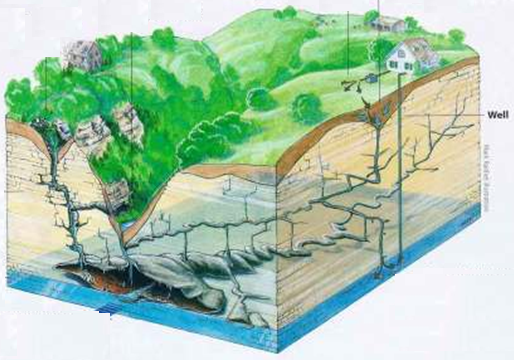
\includegraphics[width=0.37	\textwidth]{Figs_QE/reservoir3D_1}

		\caption{Example of a \emph{3-D} geological reservoir.}
		\label{fig:example3Dreservoir}
		\end{figure}

The limited access to measurements of the variables of interest makes any inference attempt very challenging. The aforementioned sampling problem implies that geophysical inverse problems are typically undetermined. In particular, characterizing a reservoir is based on the use of several sources of information, such as: \emph{wells} (direct samples), production data, and seismic data \cite{Oliver_2008_a,GuyagulerBaris2002_a,krause08efficient,olea_84_a}. 

On the one hand, \emph{Seismic data} is usually available at large scale, provided even through the entire reservoir. However, the related data is sampled on coarser grids and associated with several uncertainties and noise levels. On the other hand, \emph{Well observations} consist on well logs taken from process as described in Fig. \ref{fig:samplingWell}. \emph{Well data} is only available in areas of measurement provided by the existing wells. However, \emph{wells} are sampled on a fine grid in the paths of interest providing better details than seismic data and the uncertainty associated with these measures is smaller than the seismic sources.


		\begin{figure}
		\centering
		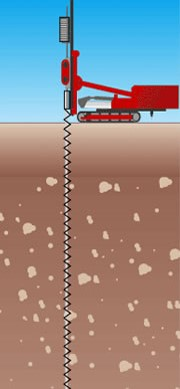
\includegraphics[width=0.12	\textwidth]{Figs_QE/sondaje1}
		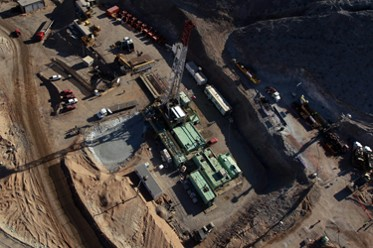
\includegraphics[width=0.37	\textwidth]{Figs_QE/sondaje2}

		\caption{Sampling scheme.}
		\scriptsize{Left: Example of a well sampling scheme. Right: Example of an actual well sampling system.}
		\label{fig:samplingWell}
		\end{figure}

In the case of \emph{production data}, the information is acquired along the production process in \emph{production wells}. This kind of data takes into account global factors related with features of reservoir that makes a great difference with the other sensing modalities. \emph{Historical data} considers scenarios with large volume of information collected allowing history matching approaches \cite{ katanidis_1997_a, Oliver_2008_a, Scheidt2009_a} and moving away from the scope of this thesis proposal.



\subsection{Geosciences and Uncertainty}

As it was mentioned before, the information sources for reservoir characterization contain uncertainties \cite{Onwunalu09,GuyagulerBaris2002_a,wellmann2013information}. Therefore, several techniques have been developed in order to estimate, quantify, and represent these uncertainties \cite{Bangerth04onoptimization,krause08efficient}. 

Unfortunately, the access to true observations of the subsurface structures is not possible because direct measurements are limited in number and unevenly distributed. Based on the above, the geological characterization is performed by using several indirect acquisition processes \cite{katanidis_1997_a,Oliver_2008_a}. In this context, a stochastic modeling of the problem is essential. It should also be noted that measurements may be inaccurate making the characterization of reservoirs even a harder problem \cite{Bangerth04onoptimization}.

Reservoir properties at various grid locations (pixels on a discrete two dimensional representation) are largely unknown, hence each property of interest at every grid block (or pixel) is modeled as a random variable whose variability is described by a probability measure. The reservoir characterization relies not only on reduced portion of available data but also in its placement. This rises the importance of the optimal sensing placement problem and recovery approaches for the inverse problem in Eq. \eqref{eq:Eq_Sensing_General_Noise_Sampling}, which is the focus of this work.



































































\section{Problem Statement}

\subsection{Motivation}

In this thesis proposal, the focus is on the field characterization of subsurface structures from spatial observations and its relationship with \emph{sampling theory} and \emph{inference strategies}. 

The \emph{Geosciences} global outcome correspond to the characterization of an unknown complex reservoir field. However, on account of the high number of structures, facies and properties in the subsurface, \emph{geologists} study the field through the description of its individual components. Thus, we focus on the recovery of a single subsurface property described by a \emph{2-D} regularized variable sampled in the spatial domain. The characterization of these kinds of structures is relevant for mineral prospecting, mining planning, and production stages where the number of available observations is severely restricted by technical and economic factors. Based on the above, the integration of adaptive sensing schemes and an appropriate inference methodology is a promising solution to improve classical geostatistical analysis.

Beyond prospecting processes, both exploitation by mineral blasting and short-term mine planning consider and could take advantages of sensing design for inference. While blast hole drilling systems has been focused on efficient drilling instead of high precision sampling, short term mine planning use a medium scale sampling to choose mining units based on estimated distribution of ore and waste. Units classified as ore will be sent to the plant while waste units will be sent to the waste dump. Mistakes in this classification process has a significant impact in economic terms.

%Design of blast hole drilling and short term mine planning has been stated as structured grid sampling where the degrees of freedom only consider the scale of the grid. In this context our sensing design and inference approaches could improve decision-making issues in mining units classification.

%The models and scenarios that have up until now been proposed as part of the data base are of major importance and relevance to the economic reality of Chile. In Chile, these reservoir characterization related processes are key in prospecting, exploration and exploitation of natural resources.


\subsection{Channelized Structures}

This proposal explores a classical geosciences scenario related with subsurface channels systems. As previously shown in Fig. \ref{fig:example3Dreservoir}, several continuous or discrete variables could be modeled by channelized structures. In addition, a statistical model is required as part of the forward model describing the channelized structures, where non-stationary assumption could be necessary to reproduce channel-like features \cite{Oliver_2008_a,Remy_2009_a}. In particular, our model of interest corresponds to a binary permeability channel (Fig. \ref{fig:2Dpermeabilityfield}). %Structural geological models (an essential tool in reservoir characterization studies, exploration and prospecting) are used to describe this kind of fields by map estimation and map making tasks.

		\begin{figure}[H]
		\centering
		
\includegraphics[width=0.2	\textwidth]{Figs_QE/ImagenOriginal}

		\caption{Binary permeability channel.}
		\scriptsize{Example of a \emph{2-D} representation of a binary channelized permeability field.}
		\label{fig:2Dpermeabilityfield}
		\end{figure}



 Formally, our image model is a numerical representation of the spatial distribution of a subsurface  attribute (such as thickness, permeability, porosity, flow rate, etc.) \cite{katanidis_1997_a, Lam_1983_a, Matheron_1971_a}. The general process of image reconstruction or characterization (i.e. inference of the spatial distribution) is described in Fig. \ref{fig:2DpermeabilityIP}, where given a reduced number of observations the final goal is to infer the underlying media or at least a related significant feature (such as first and second order statistics, connectivity, or transport metrics).


		\begin{figure}[H]
		\centering
		\begin{tikzpicture}
				\node[inner sep=0pt] (Original) at (0,-3)
						{
\includegraphics[width=.3\textwidth]{Figs_QE/ImagenOriginal}};
					
				\node[inner sep=0pt] (Sampled) at (4,-3)
						{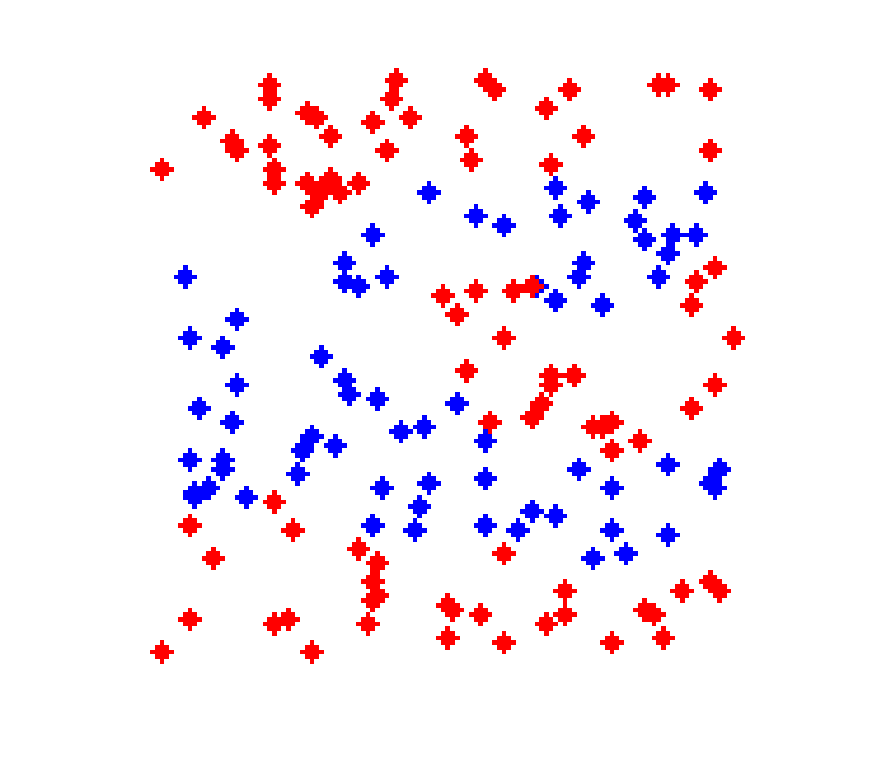
\includegraphics[width=.3\textwidth]{Figs_QE/ImagenMuestreada3}};
					
				\node[inner sep=0pt] (Infered) at (8,-3)
						{
\includegraphics[width=.3\textwidth]{Figs_QE/ImagenInferida}};
					
				\draw[->,thick] (1.15,-3) -- (1.43,-3);
				\draw[->,thick] (2.6,-3) -- (2.87,-3);

				\draw[->,thick] (5.15,-3) -- (5.43,-3);
				\draw[->,thick] (6.6,-3) -- (6.87,-3);

				\node[fill=blue!10,text width=0.9cm, text centered] (Sampled) at (2,-3) {\tiny{ Sampling System}};

				\node[fill=blue!10,text width=0.9cm, text centered] (Infered) at (6,-3) {\tiny{ Inference System}};

	\end{tikzpicture}
		\caption{Basic inverse problem scheme.}
		\scriptsize{Example of a basic scheme of inverse problem related with \emph{2-D} channelized structures characterization.}
		\label{fig:2DpermeabilityIP}
		\end{figure}






%  \textit{Geostatistics} \ref{secSecGeoIntro}, Sensing design 
%\ref{secSecSenIntro}, Recovery/reconstruction methods \ref{secSecRecIntro}, and finally some joint based methods \ref{secSecJointIntro}.


\subsection{Main Problem Statement}

We can assess the inverse problem of characterizing a field based on few measures through two stages. On the one hand, from the point of view of experimental design or sensing design, we can ask for the optimal sensing schemes optimizing $m << N$ observations, guiding the problem to find the best distribution for the observations in order to improve the knowledge of the original signal $\mathbf{X}$. This problem is usually termed as \emph{Optimal Sensor Placement} (\emph{OSP}) \cite{olea_84_a,krause08thesis,krause11robust}. 

On the other hand, from the point of view of the inference stage, given an appropriate sensing scheme, we can ask for best strategy to infer the field characterization from the available measures. In particular, the \emph{Geosciences} community developed several statistics tools in order to achieve good estimations for describing structures with spatial dependence such as channelized fields.











































\section{Literature Review}

In the next sections we describe the \emph{state-of-art} of the \textit{Geostatistical} approaches related with multi-point simulations (sec. \ref{secSecGeoIntro}), and sensing design based approaches (sec. \ref{secSecSenIntro}).


\subsection{Methods used in Geostatistical Analysis}
\label{secSecGeoIntro}

In recent decades, geologists have achieved realistic representations of the internal structure of reservoirs considering complex and heterogeneous geological environments through the use of \textit{Geostatistics}. \textit{Geostatistics} deal with spatially correlated data such as facies, reservoir thickness, porosity, and permeability \cite{Oliver_2008_a}. \emph{Geostatistics} tools allow to evaluate potential exploration and production zones, where a main issue is to define well locations.

The term \emph{Geostatistics} usually refers to the branch of spatial statistics that is concerned with the analysis of an unobserved  spatial  phenomenon $Z = \{Z_{(u,v) } : (u,v) \in D \subset \R^2 \}$ (for the \emph{2-D} case), where $D$ denotes a geographical region of interest. When the spatial coordinates are discretized the subset $D$ is comprised by only $N$ positions allowing the representation of the field as the set $X = \{X_{i} : i \in \{1,\ldots, N\} \}$.

Geostatistics deals with stochastic processes defined in a region $D$, with $D \subset \R^d$ and considering $d= 1$, $2$, or $3$. For continuous stochastic fields, a classical assumption is that the field $X$ is modeled by a stationary and isotropic \emph{Gaussian} process, with zero mean, constant variance $\sigma^2$ and autocorrelation function $\rho(X_{i} , X_{i+h} ; \phi) = \mathds{E} \{ X_{i} \cdot X_{i + h}  \} $ given by $\rho(X_{i} , X_{i+h} ; \phi)=\rho(\parallel h \parallel;\phi)$, $\forall \{i\} \in D$.
%\break

\subsubsection{Multi-Point Simulations}

	In low acquisition rates regimes, the standard geostatistical inference involves the analysis of multiple point simulations (\emph{MPS}), which provides simulated realizations honoring hard data (direct samples) and replicating patterns from a training image \cite{Ortiz_2004_a,Remy_2009_a}. 

	Geostatistical simulations provide a powerful tool to reproduce more faithfully and realistically the spatial variability with a small numbers of measurements \cite{Remy_2009_a,Ortiz_2004_a}. A simple scheme is shown in Fig. \ref{fig:MPSExample}. Geostatistical simulations lead to reservoir models that can be constrained to geologic, seismic and production data. These models provide appropriate representations for \textit{geological heterogeneities}, and allow the integration of various types of data at different scale and precisions. In any regime of data, expert knowledge is required to validate and to interpret the applicability of the \emph{Geostatistic tools} \cite{Oliver_2008_a, BKWSS06, Bangerth04onoptimization}. 


		\begin{figure}[H]
		\centering
		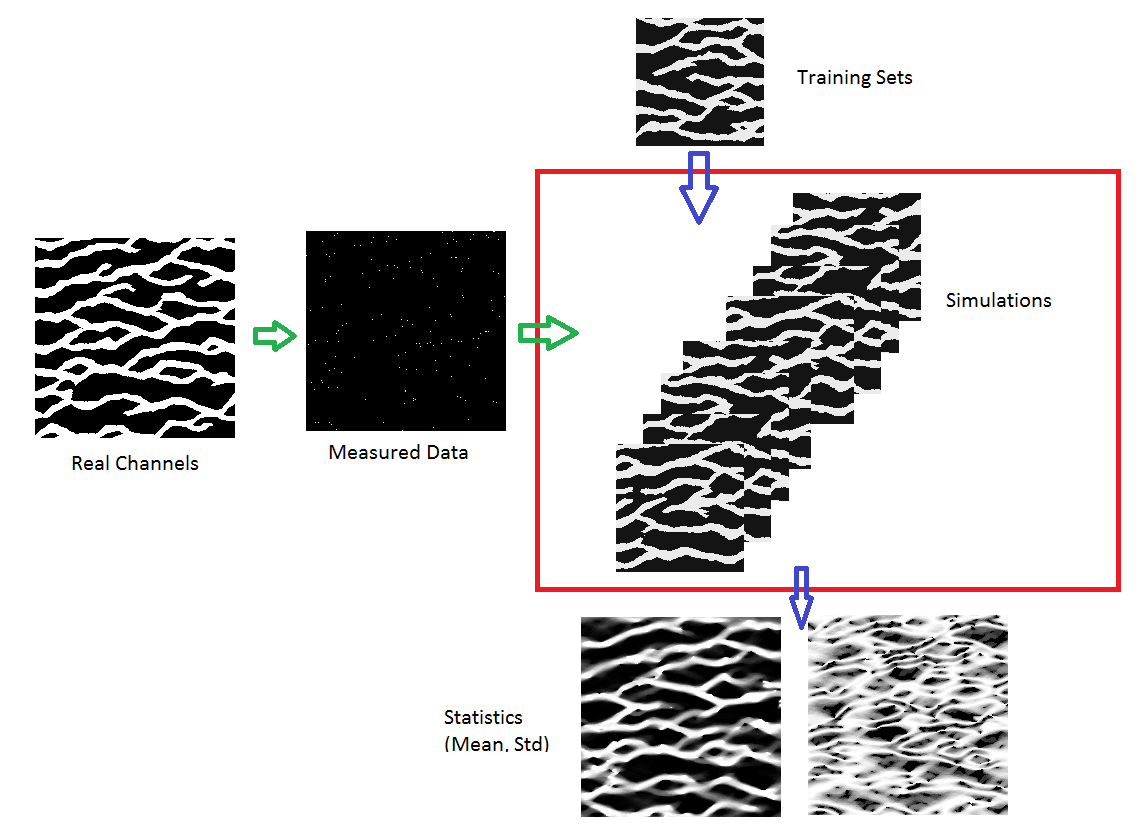
\includegraphics[width=0.7	\textwidth]{Figs_QE/Scheme.png}

		\caption{Example of a simulation based system.}
		\label{fig:MPSExample}
		\end{figure}


Deterministic \emph{Kriging} provides good solutions at data conditioning while object-based approaches provides acceptable solutions in the reproduction of geological shapes, but none method is good at both scenarios \cite{Lam_1983_a,Ortiz_2004_a,BKMPW05,olea_84_a}. Thus, multi-point simulation (\emph{MPS}) was developed to combine the strengths of previously stated approaches. The \emph{MPS} methodology recreates a realistic realization of the target field keeping the flexibility of pixel based simulation methods. At the same time, honoring well or seismic data is imposed by hard data incorporation as the initial state of the simulated media. Furthermore, \emph{MPS} realizations can reproduce complex geological shapes and structures by the estimation of simultaneous statistics at multiple positions from the training image.

	
\subsubsection{\emph{MPS} and Training Images}
\label{sec_TrainingImages}

\emph{MPS} incorporates a prior model by the use of a training image. It can be defined as a \emph{2-D} or $3-D$ valid realization of a field with the same structures that the target field (e.g. structures like channels, reefs, bars, dikes, oriented facies) representing the full range of possible shapes and its scales. Therefore, training images allow to model complex geological features and their connectivity. 

Training image must be considered as a conceptual representation of the geological field instead of an actual realization of it, providing only relative spatial information of the distribution of variables of interest in the field \cite{Scheidt2009_a}.

The generation and selection of training images is an important challenge for the \emph{MPS} methodology. A classical option is the simulation of unconditioned realizations using object-based approaches where an expert user defines the facies shapes and dimensions of interest. In order to select an appropriate training image from a set of available ones, a consistency check has been proposed to compare and validate available well data \cite{Strebelle_2004a}.

\emph{MPS} was proposed for going beyond \emph{two-point} statistics \cite{Guardiano_1993_a} using training images to describe the full range of structures present in the geological field, but due to the limited size of training images only the inference of a very reduced portion of the real \emph{multiple-point} statistics is accurate. Therefore, statistics for large scale structures are usually ignored because can led to undesired discontinuities.

	
\subsubsection{Statistics from Training Images}
\label{sec_StatsTrainingImages}

It is important to note that training images are a source of excepted patterns in the target field. For example, let $X = \{ X_{i} : i \in \{1,\ldots, N\}  \}$ be a categorical field to be simulated, with $z_0, \ldots, z_r$ different states defining the alphabet of an individual $X_{i}$ variable. The \emph{MPS} process is a one pixel at time based approach that works sequentially. In \emph{MPS}, a random path is defined to explore all the field positions to be simulated (excluding hard data positions, if available). Explored positions are then simulated becoming conditioning data for the positions to be explored later in the path sequence.

In a specific unsampled variable $X_{j}$, a context based rule is required to define the $c$ closest and most relevant context $X_S = \{ X_{S_1} = x_{S_1}, \ldots, X_{S_c} = x_{S_c} \}$. The selected variables are chosen from initial hard data and previously simulated variables. Then, the probability that the explored variable $X_{j}$ has the state $z$ given the conditioning data $X_{S}$ is estimated by the \emph{Bayes} rule:

\begin{equation}
p(X_{j} = z | X_{S} = x_{S}) = \frac{p(X_{j} = z, X_{S} = x_{S}) }{p(X_{S} = x_{S}) } .
\label{eq:bayesMPS}
\end{equation}


Both $p(X_{j} = z, X_{S} = x_{S}) $ and $p( X_{j} = z)$ are estimated from an appropriate training image. In particular, $p( X_{S} = x_{S}) = \frac{\#(x_{S})}{N}$ with $N$ the number of pixels of the training image (in this case equal to the size of the target field to be simulated), and $\#(x_{S})$ is the number of occurrences of the specific data pattern $x_{S}$ in the training image. 

The probability $p(X_{j} = z, X_{S} = x_{S}) $ can be estimated as a pattern with one additional conditioning. Then $p(X_{j} = z, X_{S} = x_{S})  =  \frac{\#(x_{S,j})}{N}$, with $\#(x_{S,j})$ the number of occurrences of the pattern including the conditioning data and the central variable $X_{j}$ with the specific value $z$. 

%Finally, the conditional probability associated to the occurrence of state $z$ at location $\{j\}$ can be estimated by:

%\begin{equation}
%p(x_{\{j\}} = z | X_{S}) = \frac{\#(x_{S,\{j\}}) }{ \#(x_{S})}
%\label{eq:bayesMPS_Final}
%\end{equation}

%Evaluating the expression \eqref{eq:bayesMPS_Final} for the $z$ possible values allows drawing a realization of the stochastic process for the explored variable.





































\subsection{Methods used in Sensing Design}
\label{secSecSenIntro}

The selection of the best set of informative observations corresponds to a common problem in different contexts such as temperature and light monitoring, sensing contamination in a river, mining exploration, collaborative robotic networks design, statistical experimental design, among others \cite{krause06near22,BKWSS06,krause08efficient,guestrin05near}. In general, this optimization problem is NP-hard, which is more critical at low acquisition rates. 


\subsubsection{Optimal Well Placement}

%In this particular case is possible to impose a discrete representation at both the available locations and the alphabet of each stochastic variable at these locations.

In our context, we focused on the scenario of pixel based measurements that model well logs. Here, the sensing design reduces to the optimal well placement (\emph{OWP}) problem. In a nutshell, \emph{OWP} problem addresses the most proper locations to make measurements. The related problem of \emph{optimal sensor placement} is an active research area in \emph{communications} \cite{krause11robust,krause09simultaneous} and \emph{machine learning} \cite{guestrin05near,krause08near}. The problem states the optimal (or near optimal) systematic way to take measurements in order to maximize the inference performance in some metric. For example, Fig. \ref{fig:sensingschemesoutcomes} presents a description of two sensing approaches in a recovery based system.


	\begin{figure}[ht!]
	\centerline{
		\begin{subfigure}[b]{0.4\textwidth}
			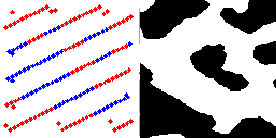
\includegraphics[width=\textwidth]{Figs_QE/malmuestreo}
		\end{subfigure}			
	}
	\vspace{-0.3cm}
	\centerline{
		\begin{subfigure}[b]{0.4\textwidth}
			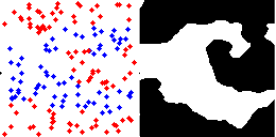
\includegraphics[width=\textwidth]{Figs_QE/buenmuestreo}
		\end{subfigure}			
	}
		\caption{Sensing design example and its effect on reconstruction of the field.}
		\scriptsize{ Upper row: an arbitrary structured sensing scheme (left) and the achieved reconstruction by the measures at this scheme locations (right). Lower row: a near optimal sensing scheme (left) and the achieved reconstruction by the measures at this scheme locations (right). The real image corresponds to the fig. \ref{fig:2Dpermeabilityfield} }
	\label{fig:sensingschemesoutcomes}
 	\end{figure}


Some approaches in the literature proposed preferential sampling schemes oriented to optimize productivity (production functionals) and economic factors \cite{Onwunalu09, BKMPW05, BKWSS06}. Several optimization methods were proposed to achieve some of these optimal functionals such as adjoint-based gradient \cite{Onwunalu09}, simultaneous perturbation stochastic approximation (\emph{SPSA}) \cite{Bangerth04onoptimization}, finite difference gradient (\emph{FDG})  \cite{Bangerth04onoptimization}, very fast simulated annealing (\emph{VFSA})  \cite{Bangerth04onoptimization}, binary genetic algorithm (\emph{bGA})  \cite{Onwunalu09}, continuous or real-valued GA (\emph{cGA}) \cite{Onwunalu09}, and particle swarm optimization (\emph{PSO}) \cite{Onwunalu09}.

While these factors are important in the industrial scenario, the idea of global uncertainty reduction could have a positive impact, directly or indirectly, on the improvement of these other practical factors \cite{krause06near22}. In this context, Wellman \cite{wellmann2013information} proposed the use of \emph{information theoretic} tools in the geostatistical analysis for map making tasks. In this specific case, there is a direct connection with \emph{conditional entropy} and its applicability to the characterization of the uncertainty of regionalized variables. On the theoretical side, Wellman \cite{wellmann2013information} shown that, in a categorical stochastic field, the regionalized variables with higher \emph{conditional entropy} are located in the facies transition zones.

%Therefore, the use of reconstruction metrics (RMSE, SNR, etc) or Uncertainty measures (Shannon Entropy). 


















































































































































%\end{intro}